\documentclass[dvipdfmx,11pt]{beamer}

% 数式
\usepackage{amsmath,amssymb,bm} %数式環境
\usepackage{mathtools}
\usepackage{physics}
\usepackage{autobreak}
\usepackage{tikzsymbols}

% 画像
\usepackage{graphicx}
\usepackage[dvipdfmx]{color}

% 脚注
\usepackage[hang,small,bf]{caption}

% 括弧
\newcommand{\Bigparen}[1]{\Bigl(#1\Bigr)}
\newcommand{\Bigbrace}[1]{\Bigl\{#1\Bigr\}}
\newcommand{\Bigbrac}[1]{\Bigl[#1\Bigr]}
\newcommand{\Biggparen}[1]{\Biggl(#1\Biggr)}
\newcommand{\Biggbrace}[1]{\Biggl\{#1\Biggr\}}
\newcommand{\Biggbrac}[1]{\Biggl[#1\Biggr]}

\usefonttheme{professionalfonts} %数式フォントをいつも通りにする
\usetheme{metropolis} % Use metropolis theme



\title{}
\author{}
\date{\today}
\institute{所属機関}
\begin{document}
\maketitle

\begin{frame}{目次}
  \tableofcontents
\end{frame}


\section{セクション1}

\begin{frame}
  \frametitle{Introduction: The community detection from the perspective of physics}

  Approach to the community detection problem
  \begin{itemize}
    \item Min Bisection
    \begin{itemize}
      \item Optimizing the objective function (e.g. modularity) for a given network
      \item Maximizing is NP-hard but it performs well in real-world networks
      \item However, model sometimes overfits to the data 
    \end{itemize}

  \end{itemize}

    \begin{columns}
      \begin{column}{0.4\textwidth}
        \begin{figure}
          \centering
          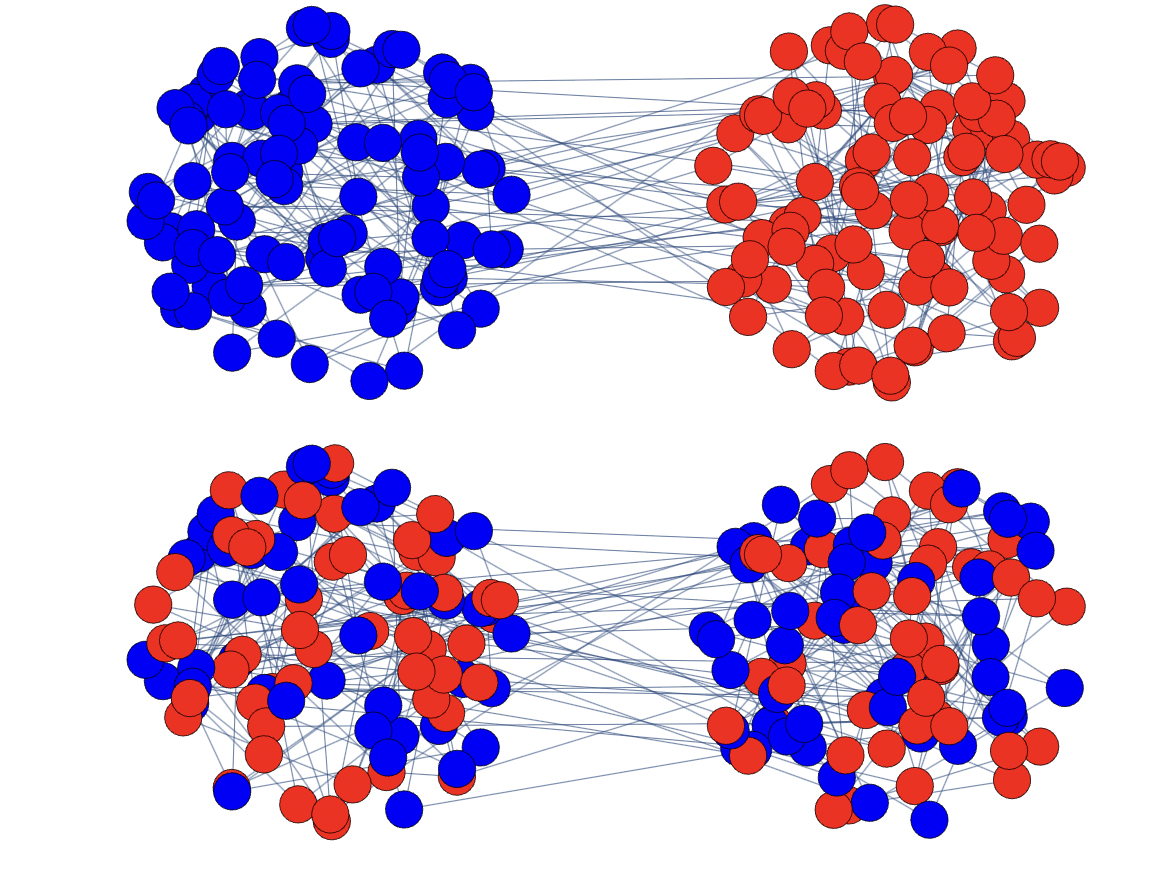
\includegraphics[width=0.8\linewidth]{figure/overfit.png}
          \caption{Partition of a random graph}
        \end{figure}
      \end{column}
  
      \begin{column}{0.60\textwidth}
        \begin{itemize}
          \item The top partition has 38 edges crossing while the bottom one has 39.
          \item For optimzer, the top one is ''optimal" but actually there is no community. 
        \end{itemize}
      \end{column}
    \end{columns}
\end{frame}



\begin{frame}
  \frametitle{Introduction: The community detection from the perspective of physics}

  \begin{itemize}
      \item In computer science, we think \alert{worst-case instances} for evaluating algorithms.
      \item However, the real world networks are rarely worst-case instances.
      \item In physics, we think \alert{typical instances} for evaluating models. (e.g. thermodynamics) \\
      $\Rightarrow$ It is natural to use physical perspective to evaluate the community detection models.
  \end{itemize}
\end{frame}



\begin{frame}
  \frametitle{二段組}

  \begin{columns}
    \begin{column}{0.48\textwidth}
        \begin{itemize}
          \item 文字
          \item 表
        \end{itemize}
    \end{column}

    \begin{column}{0.48\textwidth}
        \begin{figure}
          \centering
          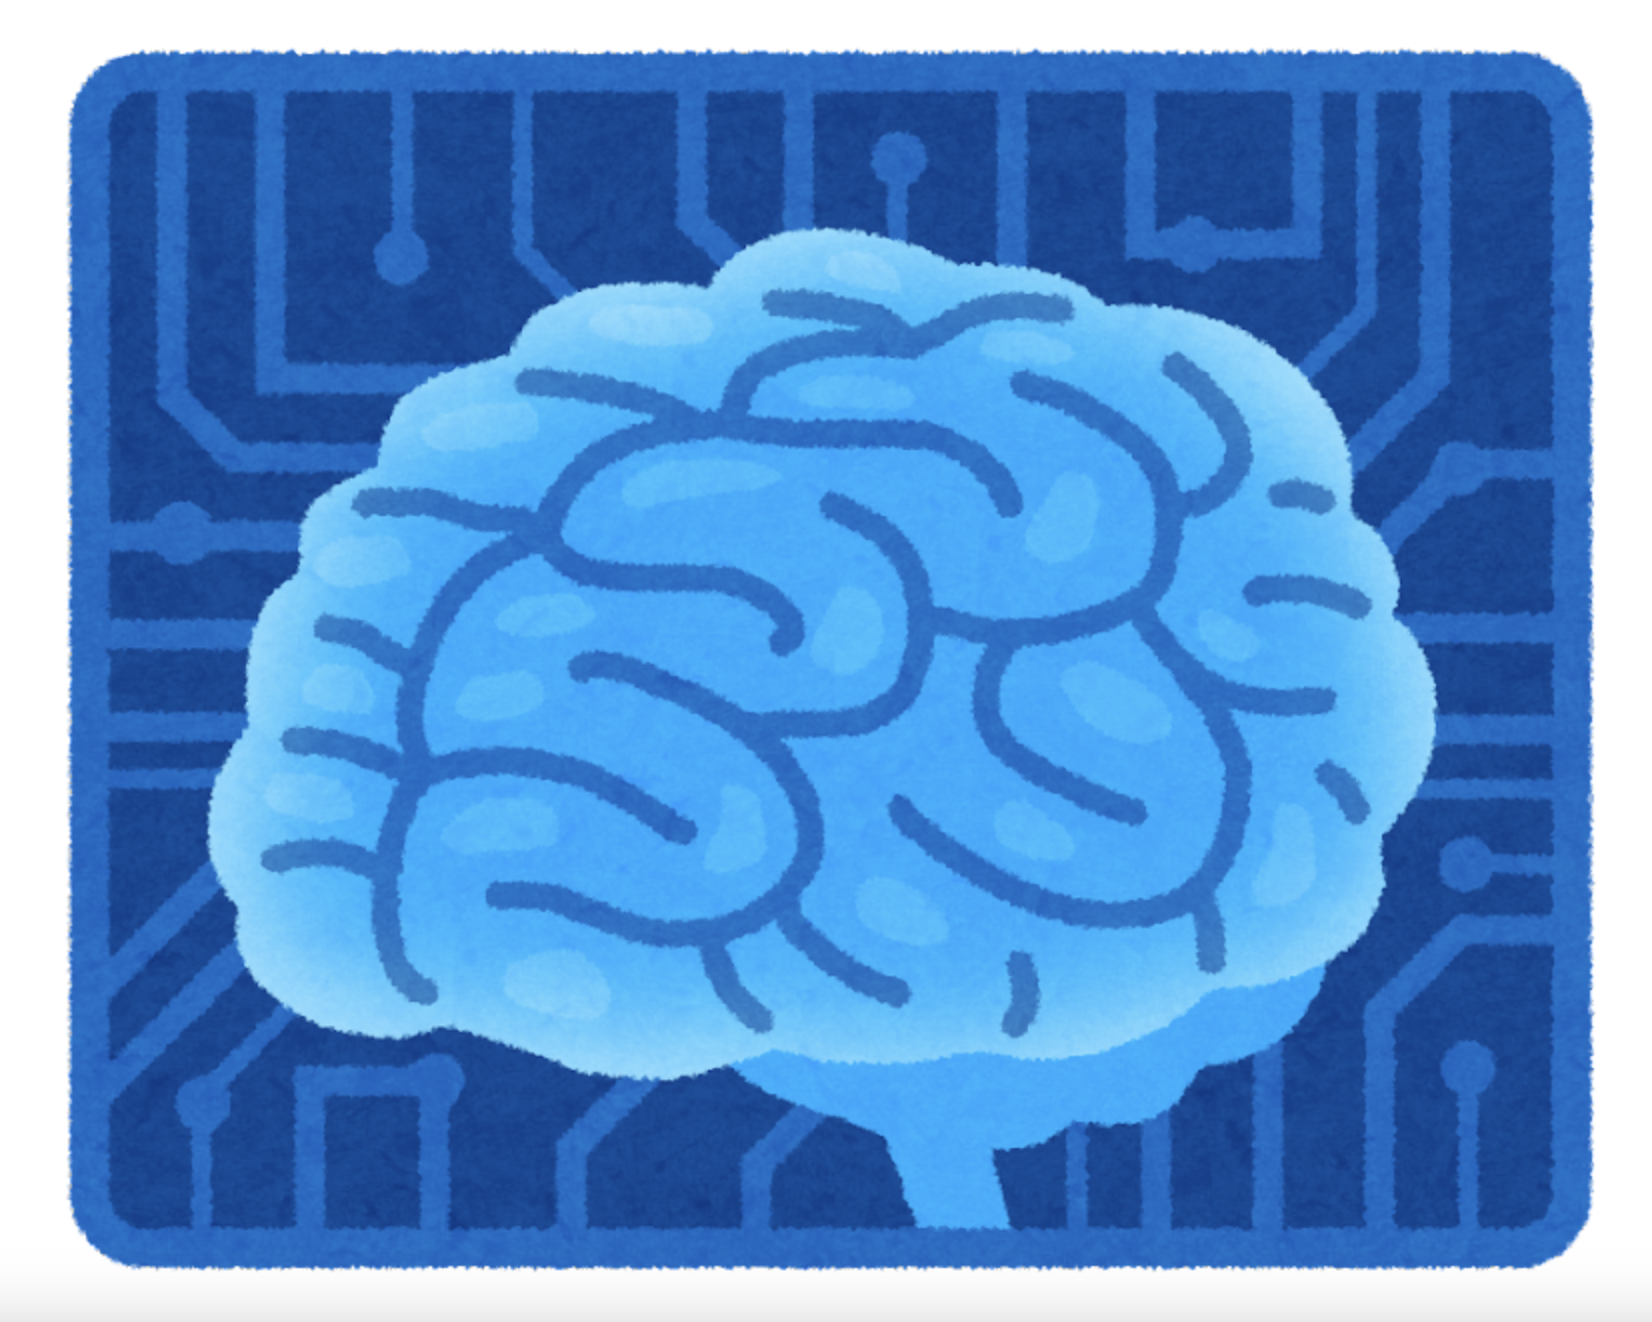
\includegraphics[width=0.8\linewidth]{figure/sample.png}
          \caption{図}
        \end{figure}
    \end{column}
  \end{columns}


\end{frame}


\begin{frame}
  \frametitle{Problem setting}
  \begin{itemize}
    \item Sparse and symmetric stochastic block model (SBM)
    \begin{itemize}
      \item $n$:  $\#$ nodes
      \item $q$:  $\#$ communities
      \item each node $i$ belongs to a community $\sigma_i \in \{1, \dots, q\}$
      \item if $i$ and $j$ belong to the same community, $A_{ij} \sim \text{Bern}(p_{in})$
      \item if $i$ and $j$ belong to different communities, $A_{ij} \sim \text{Bern}(p_{out})$
      \item $p_{in} = c_{in} / n$ and $p_{out} = c_{out} / n$ where $c_{in}$ and $c_{out}$ are constants.
    \end{itemize}
    \item In this model, the expected degree of each vertex is 
    \begin{align}
      c = \frac{n}{q} \times {p_{in}} + \qty(1-\frac{n}{q})\times{p_{out}} = \frac{c_{in} + (q-1) c_{out}}{q}
    \end{align}
    \item Note that Eronds-Renyi model is a special case of SBM where $G(n, p=c/n)$.
\end{itemize}
\end{frame}

\begin{frame}
  \frametitle{Goal}
  There are several types of goal in the community detection problem when $G$ generated from SBM is given.
  \begin{itemize}
    \item \alert{Exact reconstruction}: Finding the planted assignment exactly up to a global permutation.
    \item \alert{Reconstruction (weak recovery)}: Finding the planted assignment whose accuracy is better than random guess ($1/q$).
    \item \alert{Detection}: Hypothesis testing whether $G$ is generated from SBM or Eronds-Renyi model.
  \end{itemize}
  In this talk, we assume $c_{in}$ and $c_{out}$ are known and focus on the reconstruction and detection problems, which are strongly analogous to physics.
\end{frame}

\begin{frame}
  \frametitle{Preparation: Statistical physics and Ising model}
  \begin{itemize}
    \item Statistical physics is a study of macroscopic properties of a system from microscopic properties.
    \item \alert{Ising model}: a simple but fundamental model of magnetism and phase transition.
    \begin{itemize}
      \item There are $n$ atoms on a lattice $G = (V, E)$ and each atom has a spin $\sigma_i \in \{-1, 1\}$.
      \item Neighboring atoms tend to align their spins, so the energy of the system is
      \begin{align*}
        H(\sigma) = - J \sum_{(i, j) \in E}  \delta_{\sigma_i, \sigma_j}.
      \end{align*}
      \item The probability of the system in equilibrium is given by the Boltzmann distribution
      \begin{align*}
        P(\sigma) \propto \exp(- H(\sigma) / T) = \exp( \frac{J}{T} \sum_{(i, j) \in E}  \delta_{\sigma_i, \sigma_j}),
      \end{align*}
      where $T$ is the temperature.
    \end{itemize}
  \end{itemize}
\end{frame}

\begin{frame}
  \frametitle{Preparation: Statistical physics and Ising model}
  There is a \alert{phase transition} in the Ising model, which is a sudden change of the macroscopic properties of the system.
  \begin{figure}
    \centering
    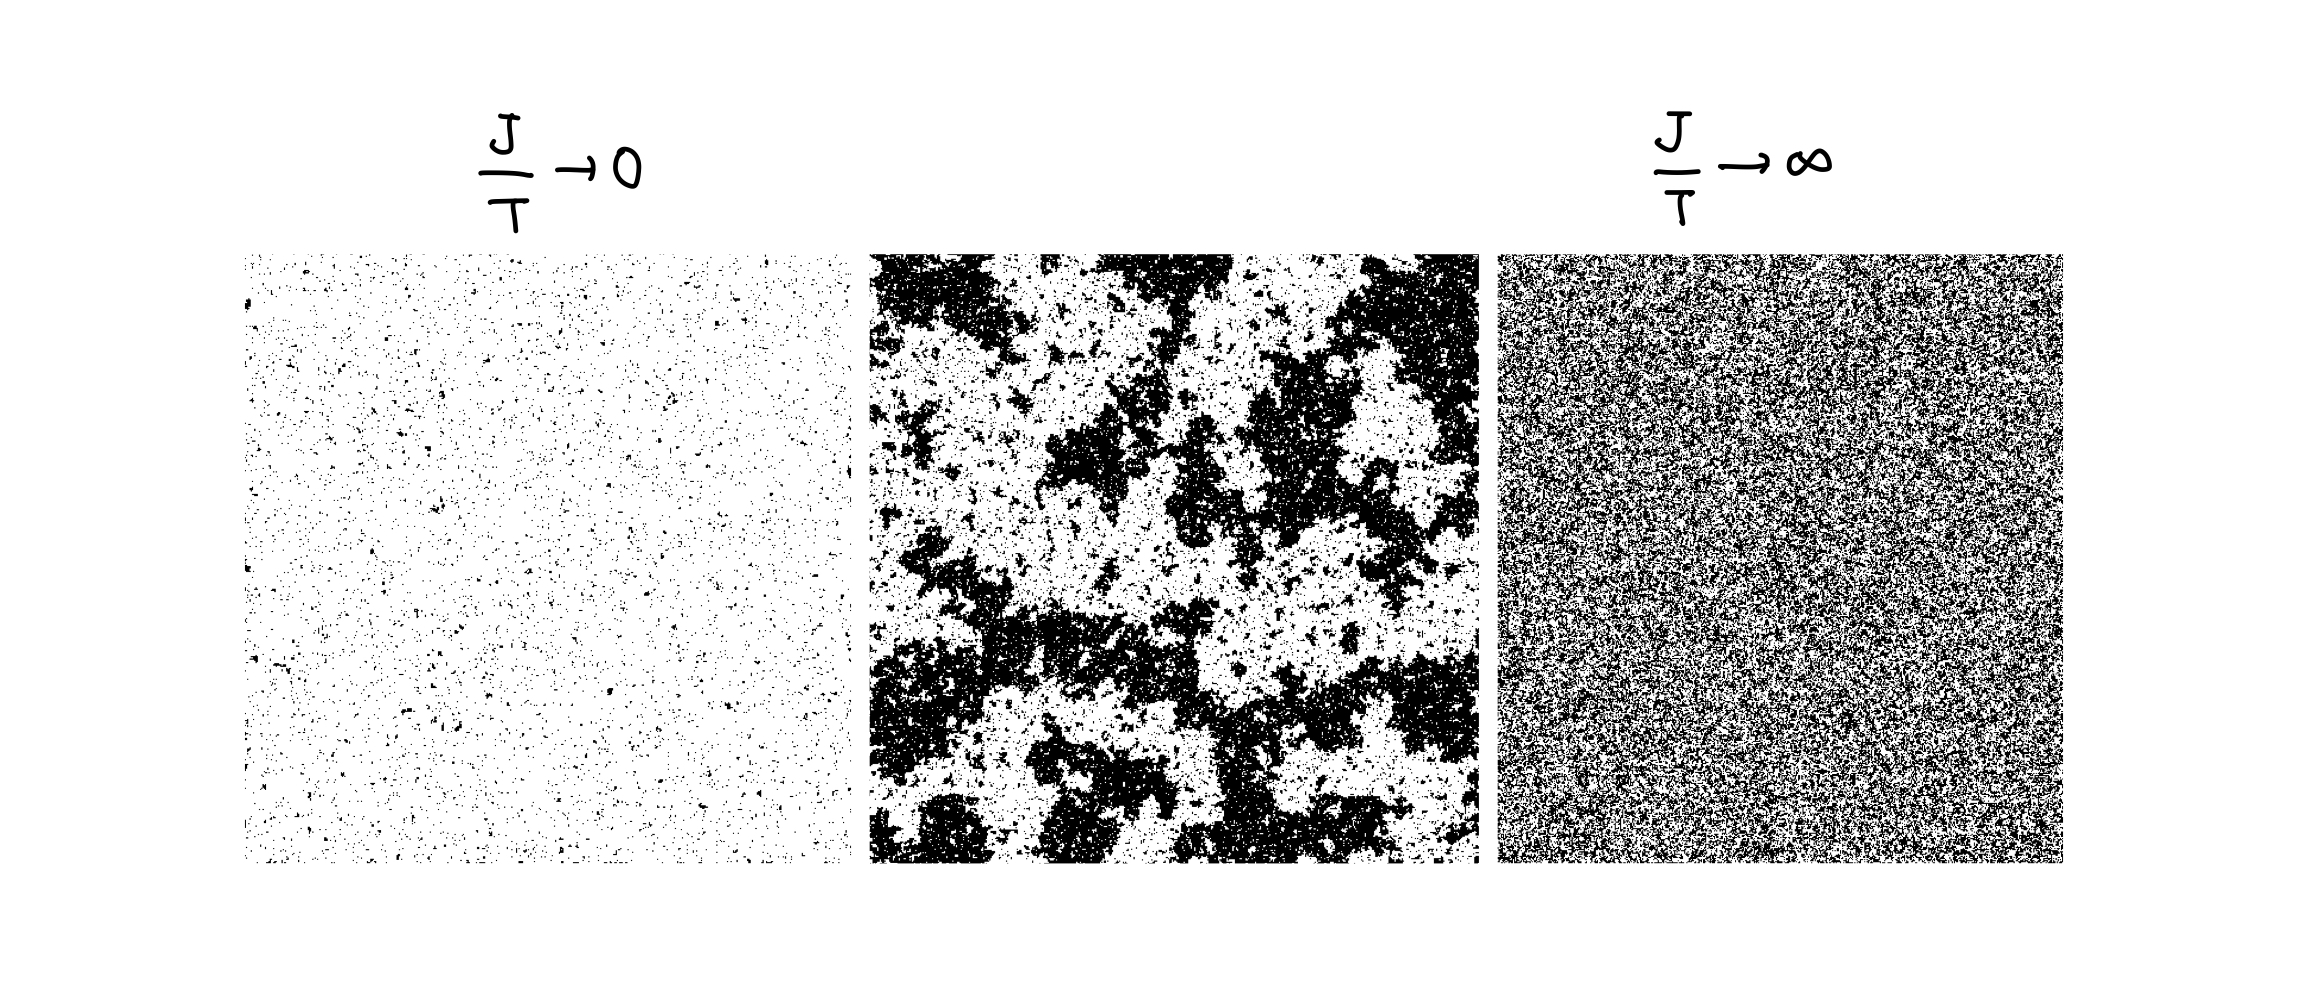
\includegraphics[width=0.6\linewidth]{figure/ising.jpeg}
    \caption{A typical states of the Ising model}
  \end{figure}
  \begin{itemize}
    \item When $J$ is large, the system is in the \alert{ferromagnetic phase} where the spins are aligned.
    \item When $J$ is small, the system is in the \alert{paramagnetic phase} where the spins are randomly distributed.
    \item The change between these phases is sudden: \alert{phase transition}.
  \end{itemize}
  
\end{frame}

\begin{frame}
  \frametitle{Community detection as a statistical physics problem}
  In our model, the probability distribution of $\sigma$ is given by
  \begin{align*}
    & ~~~~ P(\sigma \mid G) \\
    &\propto P(G \mid \sigma) \\
    & = \prod_{(i, j) \in E}  p_{\sigma_i, \sigma_j} \prod_{(i, j) \notin E} (1 - p_{\sigma_i, \sigma_j}) \\
    & = \prod_{(i,j) \in E} \qty(\frac{p_{in}}{p_{out}})^{\delta_{\sigma_i, \sigma_j}} \prod_{(i, j) \notin E}   \qty(1 - \frac{p_{in}}{p_{out}})^{1 - \delta_{\sigma_i, \sigma_j}} \\
    & = \exp(\log(\frac{p_{in}}{p_{out}}) \sum_{(i, j) \in E}  \delta_{\sigma_i, \sigma_j} + \log(1 - \frac{p_{in}}{p_{out}}) \sum_{(i, j) \notin E}  (1 - \delta_{\sigma_i, \sigma_j})) \\
    & \sim \exp(\log(\frac{p_{in}}{p_{out}}) \sum_{(i, j) \in E}  \delta_{\sigma_i, \sigma_j} )
  \end{align*}
\end{frame}

\begin{frame}
  \frametitle{Community detection as a statistical physics problem}
  \begin{itemize}
    \item In conclusion, \alert{the community detection problem is equivalent to the Ising model} with $J/T = \log(\frac{p_{in}}{p_{out}})$ in a simple approximation.
    \item From an analogy of the phase transition in the Ising model, we can expect the \alert{success-to-failure phase transition} in the community detection.
    \item Considering only the MLE is not enough to understand the properties of magnetism, which is the same for the community detection.
  \end{itemize}
\end{frame}

\begin{frame}
  \frametitle{Technical tools: Belief propagation}
  \begin{itemize}
    \item \alert{Belief propagation} (BP): method in statistical physics for computing marginal distributions $p(\sigma_i \mid G)$ of a graphical model.
    \item Sketch of BP procedure
    \begin{itemize}
      \item \alert{message}: $m_{i \to j}(\sigma_j)$ is the probability of $\sigma_i$ if $j$ does not exist. 
      \item If we know the messages $m_{1 \to 4}$ and $m_{2 \to 4}$, we can compute the message $m_{4 \to 3}$ by
      \begin{align*}
        m_{4 \to 3}(\sigma_3) \propto \qty(\sum_{\sigma_1} m_{1 \to 3}(\sigma_1)f(\sigma_1, \sigma_3)) \qty(\sum_{\sigma_2} m_{2 \to 3}(\sigma_2)f(\sigma_2, \sigma_3))
      \end{align*}
      where $f(\sigma_1, \sigma_3)$ is the relative probability of $\sigma_1$ and $\sigma_3$.
    \item If we can compute all the messages, we can compute the marginal distribution $p(\sigma_i \mid G)$ by
    \begin{align*}
      p(\sigma_3 \mid G) \propto \prod_{j \in \{1,2,4\} } \sum_{\sigma_j} m_{j \to 3}(\sigma_3) f(\sigma_3, \sigma_j)
    \end{align*}

    \end{itemize}

  \end{itemize}

\end{frame}

\begin{frame}
  \frametitle{Technical tools: Belief propagation}
\begin{itemize}
  \item If the model is tree, BP is exact.
  \item In general, we need to propagate the messages for several times until convergence.
\end{itemize}

\metroset{block=fill}

\begin{block}{Question}
  When does BP converge to the ``correct answer''?
\end{block}
\begin{itemize}
  \item $m_{i \to j}(\sigma_j=r) = 1/q$ is a trivial fixed point, where $p(\sigma_i \mid G)$ = 1/q.
  \item If BP is stacked at this fixed point, BP is no better than random guess.
  \item One can calculate the stability of fixed points by linearizing the BP equation. 
\end{itemize}

\end{frame}

\begin{frame}
  \frametitle{Sketch of stability analysis}
  \begin{itemize}
    \item Suppose the messages are almost uniform:
    \begin{align*}
      m_{i \to j}(\sigma_j) = \frac{1}{q} + \epsilon_{i \to j}(\sigma_j)
    \end{align*}
    \item Substituting this into the BP equation, we obtain in the first order of $\epsilon_{i \to j}$,
    \begin{align*}
      \epsilon^{(l+1)} \propto M \epsilon^{(l)}
    \end{align*}
    If $M$ has an eigenvalue whose absolute value is larger than 1, $\epsilon^{(l)}$ diverges. \\
    $\Rightarrow$ trivial fixed point is unstable \Smiley.
  \end{itemize}
\end{frame}

\begin{frame}
  \frametitle{Sketch of stability analysis}
  \begin{itemize}
    \frametitle{Sketch of stability analysis}
    \item From some technical calculation, we obtain
    \begin{align*}
      M = B \bigotimes T
    \end{align*}
    where 
    \begin{align*}
      T = \frac{1}{qc}
        \begin{pmatrix}
        c_{in} & \cdots & c_{out} \\
        \vdots & \ddots & \vdots \\
        c_{out} & \cdots & c_{in}
        \end{pmatrix}
    \end{align*}
    and 
    \begin{align*}
      B_{(i,j),(k,\ell)} = 
        \begin{cases} 
        1 & \text{if } \ell = i \text{ and } k \neq j \\
        0 & \text{otherwise}.
        \end{cases}
    \end{align*}
  \end{itemize}
  

\end{frame}

\begin{frame}
  \frametitle{Sketch of stability analysis}
  \begin{itemize}
    \item The relevant first eigenvalue of $T$ is given by 
    \begin{align*}
      \lambda = \frac{c_{in} - c_{out}}{qc}
    \end{align*}
    and the relevant first eigenvalue of $B$ is given by $\max(c\lambda, \sqrt{c})$.
    \begin{figure}
      \centering
      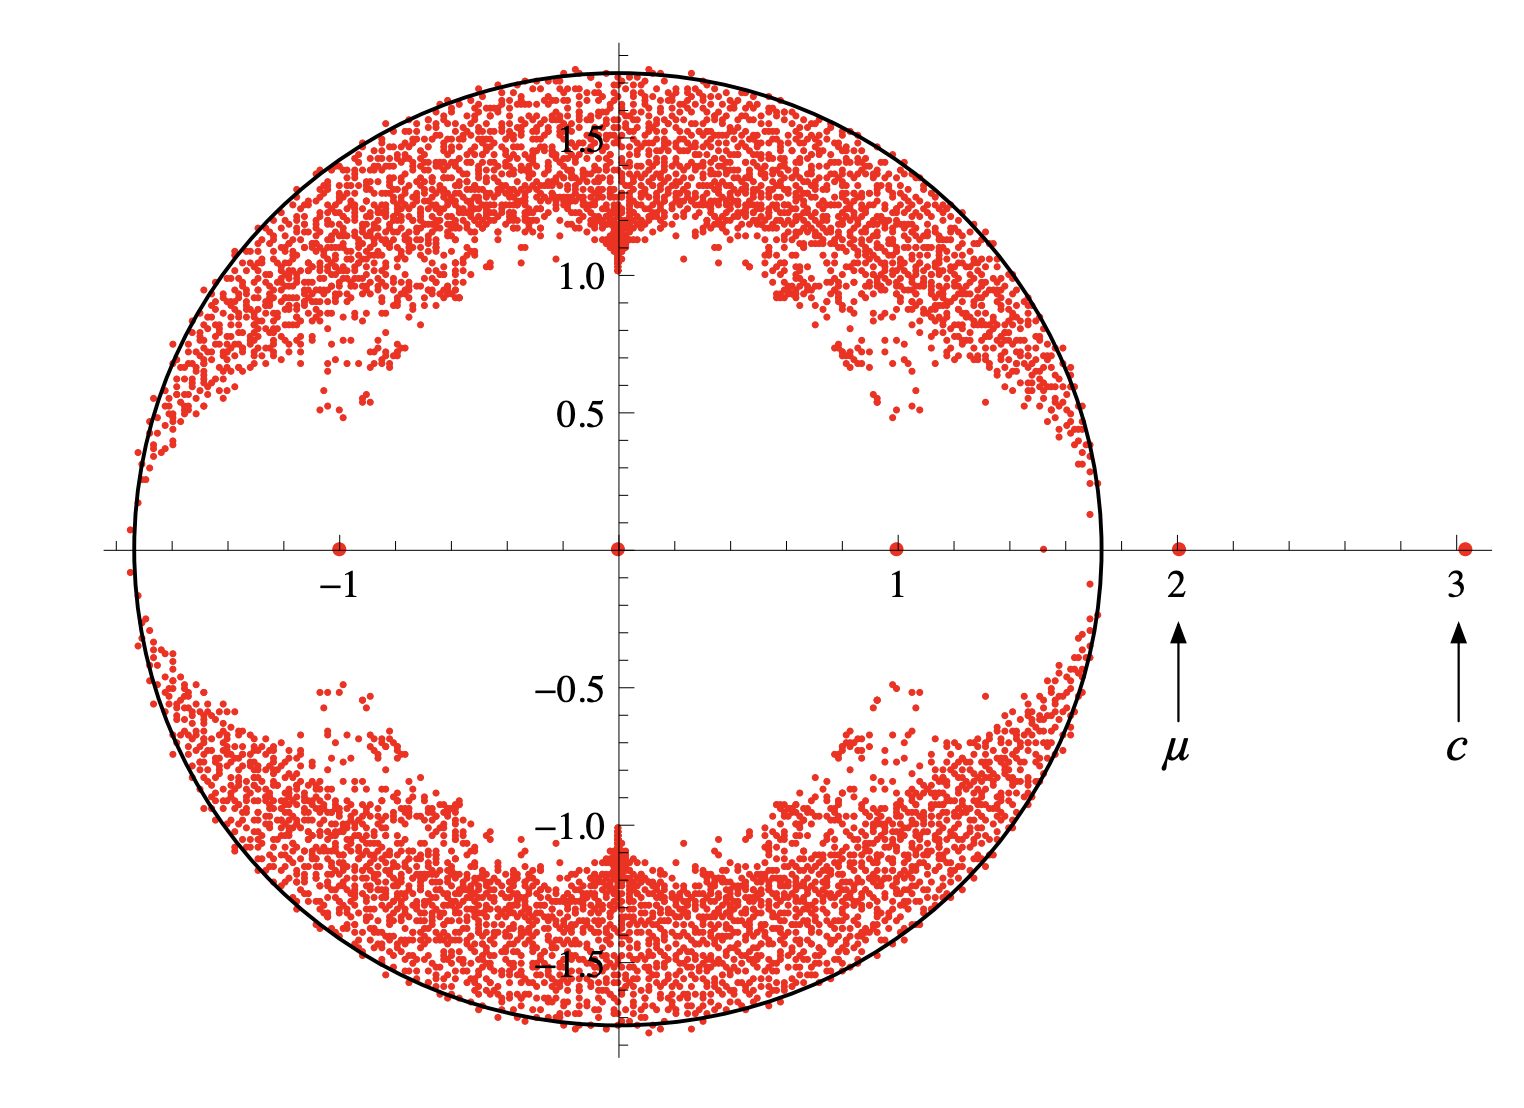
\includegraphics[width=0.3\linewidth]{figure/eign.png}
    \end{figure}
  \end{itemize}
  which leads to the following theorem.

  \metroset{block=fill}

\begin{block}{Kesten-Stigum threshold}
  If $c\lambda^2 > 1$, the trivial fixed point is unstable.
\end{block}
It is proofed that in this regime, an efficient algorithm for weak reconstruction exist \Smiley.
  

\end{frame}

\begin{frame}
  \frametitle{Contiguity}
  So far, we found ``easy regime'' of weak reconstruction.
  \begin{figure}
    \centering
    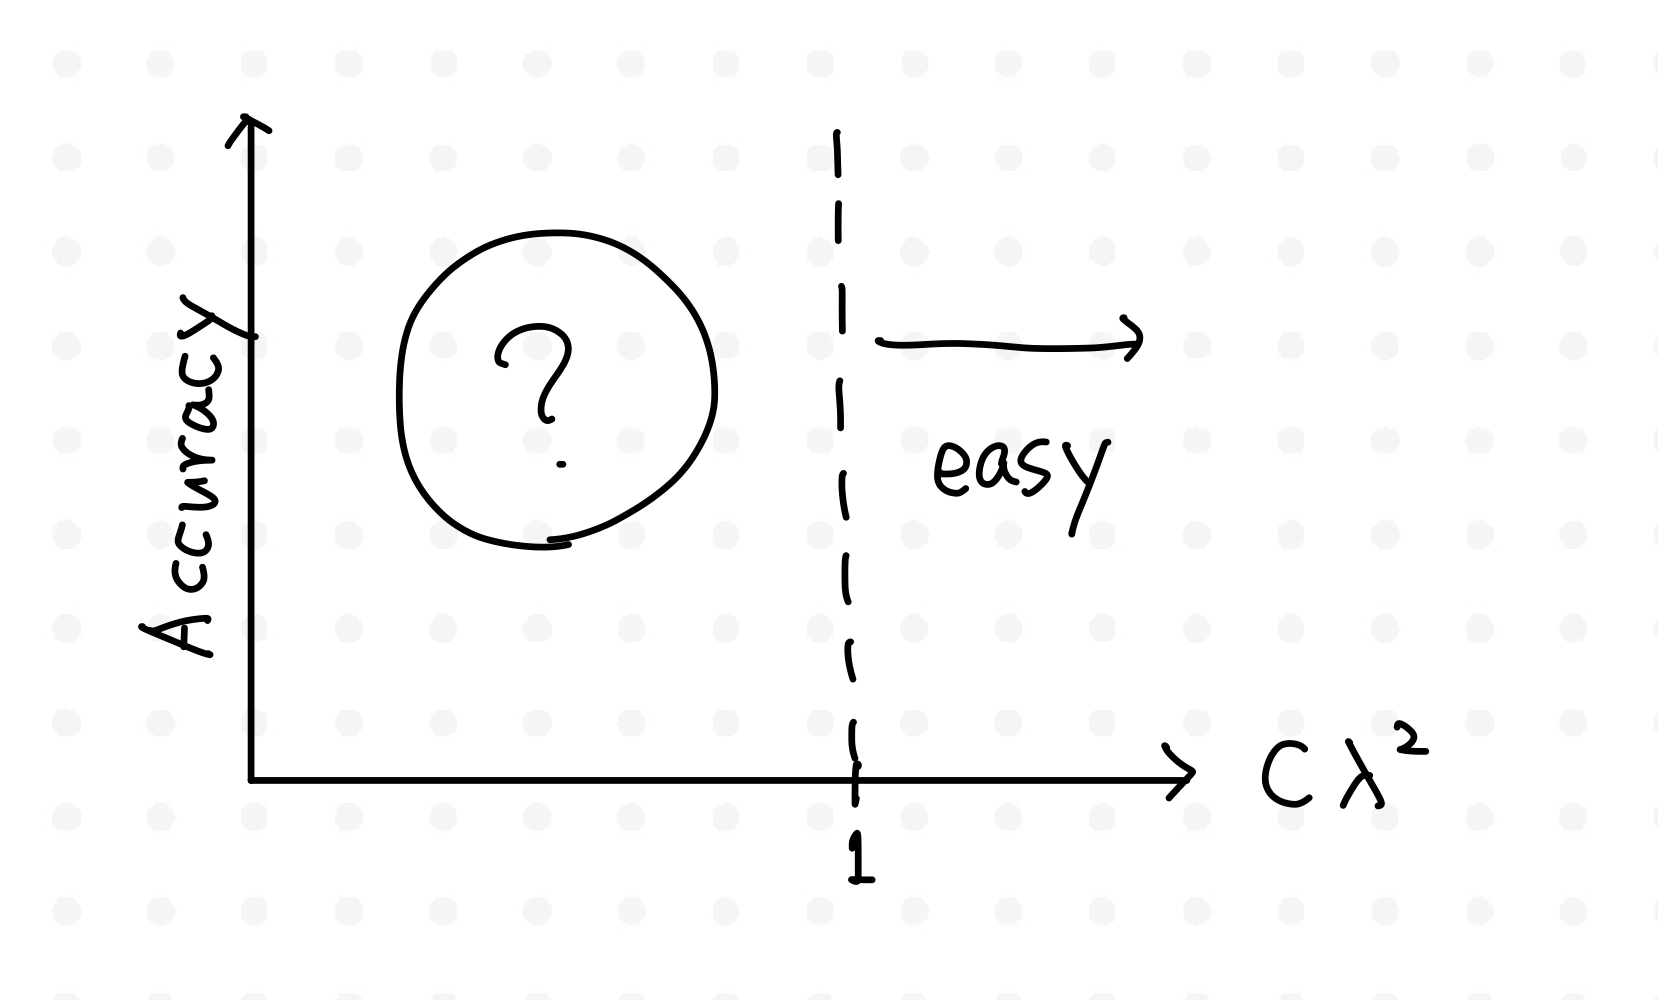
\includegraphics[width=0.5\linewidth]{figure/phase1.jpeg}
    \caption{Phase diagram of the community detection}
  \end{figure}
  \metroset{block=fill}
  \begin{block}{Question}
    Is there any regime where the weak reconstruction is impossible by any algorithm?
  \end{block}
\end{frame}

\begin{frame}
  \frametitle{Contiguity}
  \begin{itemize}
    \item P: SBM 
    \item Q: Eronds-Renyi model
  \end{itemize}
  We write $P \trianglelefteq Q$ if $\lim_{n \to 0} Q()

  

\end{frame}




\end{document}




